\documentclass[dvipsnames]{book}

\usepackage[margin=1cm,a5paper]{geometry}

\usepackage{bold-extra}
\usepackage{polski}
\usepackage{iwona}
\usepackage[OT4]{fontenc}

\usepackage{amsmath,amssymb,amsthm}
\usepackage{pgf,tikz}
\usepackage{hyperref}

\pagestyle{empty}
\setlength{\parindent}{0pt}
\setlength{\parskip}{5pt}
\renewcommand\leq\leqslant
\renewcommand\geq\geqslant

\colorlet{maincolor}{ForestGreen}
\usepackage[most]{tcolorbox}
\usepackage{varwidth}

\newtcolorbox{tresc}[3][]{enhanced, sharp corners, boxrule=0mm, colback=maincolor!10,
colframe=black,toptitle=1mm,fonttitle=\bfseries,
colbacktitle=maincolor!25, coltitle=black,
title={Zadanie #2\hfill{\it Opracowanie: #3}},#1}

\newenvironment{problem}[3]{\newpage\begin{tresc}{#1}{#2}{#3}}{\end{tresc}}

% Dodatkowe makra

\usepackage{multicol}
\usepackage{cancel}
\usepackage{bbm}

\def\ind{\mathbbm{1}}

\def\N{\mathbb{N}}
\def\P{\mathbb{P}}
\def\E{\mathbb{E}}
\def\Z{\mathbb{Z}}
\def\Q{\mathbb{Q}}
\def\R{\mathbb{R}}

\def\nwd{\mathrm{NWD}}

\newtheorem*{lemat}{Lemat}

\usepackage{enumitem}
\setlist[enumerate,1]{label={(\alph*)},topsep=0pt}

% ------------------------------------------------------------------
% Kolorowe boxy: definicje (zielone), twierdzenia/obserwacje/wnioski (niebieskie)
% ------------------------------------------------------------------

\colorlet{defcolor}{ForestGreen}
\colorlet{thmcolor}{RoyalBlue}

\newcounter{defcnt}
\newcounter{thmcnt}

% wspólny styl boxa
\tcbset{notatkibox/.style={enhanced, sharp corners, boxrule=0mm, frame hidden,
  toptitle=0.5mm, bottomtitle=0.5mm, left=2mm, right=2mm, top=1.5mm, bottom=1.5mm,
  fonttitle=\bfseries, coltitle=black, breakable, before skip=6pt, after skip=6pt}}

% \begin{definicja}[nazwa]
\NewDocumentEnvironment{definicja}{o}{%
  \refstepcounter{defcnt}%
  \begin{tcolorbox}[notatkibox, colback=defcolor!8, colframe=defcolor!25,
    colbacktitle=defcolor!25,
    title={Definicja \thedefcnt\IfValueT{#1}{\ (#1)}}]%
}{\end{tcolorbox}}

% generator środowisk niebieskich: #1 = nazwa środowiska, #2 = etykieta
\newcommand{\newthmbox}[2]{%
  \NewDocumentEnvironment{#1}{o}{%
    \refstepcounter{thmcnt}%
    \begin{tcolorbox}[notatkibox, colback=thmcolor!8, colframe=thmcolor!25,
      colbacktitle=thmcolor!25,
      title={#2 \thethmcnt\IfValueT{##1}{\ (##1)}}]%
  }{\end{tcolorbox}}%
}

\newthmbox{twierdzenie}{Twierdzenie}
\newthmbox{obserwacja}{Obserwacja}
\newthmbox{wniosek}{Wniosek}
\newthmbox{stwierdzenie}{Stwierdzenie}
% uwaga -- żółty box, \begin{uwaga}[nazwa]
\colorlet{uwagacolor}{Dandelion}

\NewDocumentEnvironment{uwaga}{o}{%
  \refstepcounter{thmcnt}%
  \begin{tcolorbox}[notatkibox, colback=uwagacolor!15, colframe=uwagacolor!40,
    colbacktitle=uwagacolor!40,
    title={Uwaga \thethmcnt\IfValueT{#1}{\ (#1)}}]%
}{\end{tcolorbox}}

% treść zadania -- szary box, \begin{zadanie}{1.1}
\colorlet{zadcolor}{Gray}

\NewDocumentEnvironment{zadanie}{m}{%
  \begin{tcolorbox}[notatkibox, colback=zadcolor!15, colframe=zadcolor!40,
    colbacktitle=zadcolor!40,
    title={Zadanie #1}]%
}{\end{tcolorbox}}

% przykład -- bez boxa, wyróżniony nagłówkiem
\theoremstyle{definition}
\newtheorem*{przyklad}{Przykład}

\renewcommand{\qedsymbol}{$\square$}


\begin{document}

\begin{center}
  {\Large\bfseries Wykład 3 --- 2026-10-16}
\end{center}

\section*{Chwilowość i powracalność --- ciąg dalszy}

\begin{przyklad}
Rozważmy łańcuch na $S = \{A, B, C\}$ o grafie i macierzy przejścia
\begin{center}
\begin{minipage}{0.45\textwidth}
\centering
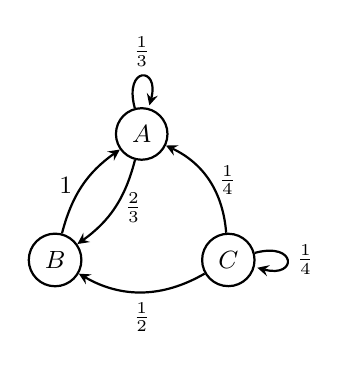
\begin{tikzpicture}[->, >=stealth, thick, node distance=2cm,
    every node/.style={font=\small},
    state/.style={circle, draw, minimum size=6mm}]
  \node[state] (A) at (0,1.6) {$A$};
  \node[state] (B) at (-1.1,0) {$B$};
  \node[state] (C) at (1.1,0) {$C$};
  \path (A) edge[loop above] node[above] {$\frac13$} (A)
        (A) edge[bend left=20] node[right] {$\frac23$} (B)
        (B) edge[bend left=20] node[left] {$1$} (A)
        (C) edge[bend right=30] node[right] {$\frac14$} (A)
        (C) edge[bend left=30] node[below] {$\frac12$} (B)
        (C) edge[loop right] node[right] {$\frac14$} (C);
\end{tikzpicture}
\end{minipage}%
\begin{minipage}{0.45\textwidth}
\[
  \mathbf{P} =
  \begin{bmatrix}
    \frac13 & \frac23 & 0 \\
    1 & 0 & 0 \\
    \frac14 & \frac12 & \frac14
  \end{bmatrix}.
\]
\end{minipage}
\end{center}
Wówczas
\begin{itemize}[topsep=0pt,itemsep=0pt]
  \item $f_{AA} = 1$, więc $A$ jest stanem powracającym,
  \item $f_{BB} = 1 - 1 \cdot \big(\tfrac13\big)^{\infty} = 1 - 0 = 1$, więc
  $B$ jest powracający,
  \item $f_{CC} < 1$, więc $C$ jest chwilowy.
\end{itemize}
\end{przyklad}

\begin{twierdzenie}
Niech $j \in S$.
\begin{enumerate}
  \item $j$ jest powracający
  \begin{align*}
    &\iff \P\big(N_j = \infty \mid X_0 = j\big) = 1 \\
    &\iff \sum_{n=1}^{\infty} p_n(j,j) = +\infty
      \quad \Big(= \E\big[N_j \mid X_0 = j\big]\Big),
  \end{align*}
  \item $j$ jest chwilowy
  \begin{align*}
    &\iff \P\big(N_j = \infty \mid X_0 = j\big) = 0 \\
    &\iff \sum_{n=1}^{\infty} p_n(j,j) < +\infty
      \quad \Big(= \E\big[N_j \mid X_0 = j\big]\Big).
  \end{align*}
\end{enumerate}
\end{twierdzenie}

\begin{proof}
Niech $i \in S$. Korzystając z ciągłości prawdopodobieństwa (zdarzenia
$\{N_j \geq k\}$ są zstępujące), mamy
\begin{align*}
  \P\big(N_j = \infty \mid X_0 = i\big)
  &= \P\Big(\bigcap_{k} \{N_j \geq k\} \,\Big|\, X_0 = i\Big)
   = \lim_{k \to \infty} \P\big(N_j \geq k \mid X_0 = i\big) \\
  &= \lim_{k \to \infty} f_{ij} f_{jj}^{k-1}
   = \begin{cases}
       f_{ij}, & f_{jj} = 1, \\
       0, & f_{jj} < 1.
     \end{cases}
\end{align*}
Ponadto
\begin{align*}
  \sum_{n=1}^{\infty} p_n(i,j)
  &= \sum_{n=1}^{\infty} \P\big(X_n = j \mid X_0 = i\big)
   = \sum_{n=1}^{\infty} \E\big[\ind_{\{X_n = j\}} \mid X_0 = i\big]
   = \E\big[N_j \mid X_0 = i\big] \\
  &= \sum_{k=1}^{\infty} \P\big(N_j \geq k \mid X_0 = i\big)
   = \sum_{k=1}^{\infty} f_{ij} f_{jj}^{k-1}
   = \begin{cases}
       \infty, & f_{jj} = 1 \ \wedge\ f_{ij} \neq 0, \\[2pt]
       \dfrac{f_{ij}}{1 - f_{jj}}, & f_{jj} < 1.
     \end{cases}
\end{align*}
Biorąc $i = j$ (wtedy $f_{jj} \neq 0$ w przypadku powracającym) dostajemy
obie równoważności.
\end{proof}

\begin{lemat}
Jeśli $i$ jest powracający i $i \to j$, to $j$ też jest powracający.
\end{lemat}

Najpierw udowodnimy pomocniczy lemat.

\begin{lemat}
Jeśli $i$ jest powracający i $i \to j$, to $j \to i$.
\end{lemat}

\begin{proof}
Udowodnimy kontrapozycję ($p \Rightarrow q$ dowodzimy jako
$\neg q \Rightarrow \neg p$). Gdyby $j \not\to i$ oraz $i \to j$, to
\[
  \P\big(T_i = \infty \mid X_0 = i\big)
  \geq \P\big(\exists_{n \geq 1}\colon X_n = j \text{ oraz } X_k \neq i
    \text{ dla } k = 1, \ldots, n-1 \,\big|\, X_0 = i\big) > 0,
\]
gdzie ostatnia nierówność zachodzi, bo $i \to j$ (a z $j$ nie da się już wrócić
do $i$). Stąd
\[
  \left.\begin{aligned} j &\not\to i \\ i &\to j \end{aligned}\right\}
  \implies
  \underbrace{\P\big(T_i = \infty \mid X_0 = i\big)}_{= 1 - f_{ii}} > 0,
\]
czyli $f_{ii} < 1$, więc $i$ jest chwilowy.
\end{proof}

\begin{proof}[Dowód lematu]
Skoro $i$ jest powracający i $i \to j$, to z lematu pomocniczego $j \to i$,
czyli istnieją $m, k$ takie, że $p_m(j,i) > 0$ i $p_k(i,j) > 0$. Wtedy
\begin{align*}
  \sum_{n=1}^{\infty} p_n(j,j)
  &\geq \sum_{n=1}^{\infty} p_{m+n+k}(j,j)
   \geq \sum_{n=1}^{\infty} p_m(j,i)\, p_n(i,i)\, p_k(i,j) \\
  &= p_m(j,i)\, p_k(i,j) \sum_{n=1}^{\infty} p_n(i,i)
   = (+) \cdot (+) \cdot (+\infty) = +\infty. \qedhere
\end{align*}
\end{proof}

\begin{wniosek}
\begin{itemize}[topsep=0pt,itemsep=0pt]
  \item Powracalność i chwilowość są własnościami klas komunikacji.
  \item Skończony łańcuch nieprzywiedlny musi być powracalny.
  \item Skończony łańcuch przywiedlny ma stan powracalny.
\end{itemize}
\end{wniosek}

\section*{Zachowanie graniczne łańcuchów Markowa}

Rozkładem $X_n$ jest $\alpha \mathbf{P}^n$ --- co się dzieje, gdy
$n \to \infty$? Najlepiej, jeśli

\begin{center}
$(*)$ \quad istnieje wektor prawdopodobieństwa $v = (v_j)_{j \in S}$
($v_j \geq 0$, $\sum_j v_j = 1$) taki, że
$\lim\limits_{n \to \infty} p_n(i,j) = v_j$ \ dla wszystkich $i,j \in S$.
\end{center}

\begin{definicja}
Wektor $v$ nazywamy wtedy \emph{rozkładem granicznym}. Gdy $|S| < \infty$,
to
\[
  \mathbf{P}^n \xrightarrow[n \to \infty]{}
  \begin{bmatrix}
    v_1 & \cdots & v_N \\
    \vdots & & \vdots \\
    v_1 & \cdots & v_N
  \end{bmatrix}
  \qquad\text{oraz}\qquad
  \lim_{n \to \infty} \alpha \mathbf{P}^n
  = \alpha \lim_{n \to \infty} \mathbf{P}^n = v.
\]
\end{definicja}

Dlaczego ,,najlepiej''? Bo $(*)$ implikuje:

\textbf{1) Stabilizację rozkładów jednowymiarowych} (ważne!). Dla każdego
$j \in S$
\begin{align*}
  \lim_{n \to \infty} \P(X_n = j)
  &= \lim_{n \to \infty} \big(\alpha \mathbf{P}^n\big)_j
   = \lim_{n \to \infty} \sum_{i \in S} \alpha_i\, p_n(i,j)
   \overset{?}{=} \sum_{i \in S} \lim_{n \to \infty} \alpha_i\, p_n(i,j) \\
  &= \sum_{i \in S} \alpha_i v_j = v_j.
\end{align*}
Zatem $(*)$ implikuje, że dla dowolnego rozkładu początkowego $\alpha$, jeśli
$X_0 \sim \alpha$, to $X_n \xrightarrow{d} v$ (\emph{zapominanie rozkładu
początkowego}).

\begin{uwaga}[Przejście z granicą pod sumę]
Gdy $|S| < \infty$, przejście oznaczone ,,$?$'' jest oczywiste. Gdy
$|S| = \infty$, korzystamy z faktu: jeśli
$(x_{i,n})_{i,n \in \N} \subset \R$ spełnia
\begin{enumerate}[label=\arabic*),topsep=0pt,itemsep=0pt]
  \item dla każdego $i$ istnieje $\lim_{n \to \infty} x_{i,n}$,
  \item $\sum_i \sup_n |x_{i,n}| < \infty$,
\end{enumerate}
to możemy przejść z granicą pod sumę (całkę). U nas
$x_{i,n} = \alpha_i\, p_n(i,j)$ oraz
\[
  \sum_i \sup_n |x_{i,n}|
  = \sum_i \sup_n \alpha_i\, p_n(i,j)
  = \sum_i \alpha_i \sup_n p_n(i,j)
  \leq \sum_i \alpha_i = 1.
\]
\end{uwaga}

\textbf{2) Interpretację:} rozkład graniczny to graniczna średnia proporcja
czasu spędzonego przez $(X_n)_n$ w każdym ze stanów. Istotnie, dla dowolnych
$i,j \in S$
\[
  \lim_{n \to \infty}
    \E\Big[\frac1n \sum_{k=0}^{n-1} \ind_{\{X_k = j\}} \,\Big|\, X_0 = i\Big]
  = \lim_{n \to \infty} \frac1n \sum_{k=0}^{n-1}
    \underbrace{\P\big(X_k = j \mid X_0 = i\big)}_{= p_k(i,j)}
  = v_j,
\]
gdzie ostatnia równość wynika z lematu Cesàro--Stolza.

\begin{definicja}[Rozkład stacjonarny]
Niech $\pi$ będzie rozkładem prawdopodobieństwa na $S$. Mówimy, że $\pi$ jest
\emph{stacjonarny} dla $\mathbf{P}$, jeśli $\pi \mathbf{P} = \pi$.
\end{definicja}

\begin{przyklad}
\begin{itemize}[topsep=0pt,itemsep=0pt]
  \item $\mathbf{P} = \begin{bmatrix} 1 & 0 \\ 0 & 1 \end{bmatrix}$ ---
  $(*)$ nie zachodzi, a każdy $\pi$ jest stacjonarny.
  \item $\mathbf{P} = \begin{bmatrix} 0 & 1 \\ 1 & 0 \end{bmatrix}$ ---
  $(*)$ nie zachodzi, a $\pi = \big[\tfrac12, \tfrac12\big]$ jest stacjonarny.
\end{itemize}
\end{przyklad}

\end{document}
